\documentclass[10pt,a4paper]{article}
\usepackage[margin=2.1cm]{geometry}
\usepackage{amsmath,amssymb,bm}
\usepackage{graphicx,booktabs,xcolor,enumitem,hyperref}
\hypersetup{colorlinks,linkcolor=blue!50!black,urlcolor=blue!50!black}
\newcommand{\kc}{\kappa_2}
\newcommand{\note}[1]{\par\smallskip\noindent\colorbox{gray!12}{\parbox{\dimexpr\linewidth-2\fboxsep}{\small #1}}\par\smallskip}
\newcommand{\evd}[1]{\textsf{\small[#1]}}
\newcommand{\simple}[1]{\par\noindent\textbf{In simple words:} #1\par\smallskip}
\title{TOP-Q --- Days 9--10 worked notes\\[2pt]\large The bridge: does array-level protection survive inside an MZI mesh?}
\author{PH 5110 term paper --- Kotapati Kishore (EE26E016)}
\date{31 October 2026 (four days ahead of the revised plan)}
\begin{document}\sloppy\maketitle

\note{All results are \textbf{numerical simulations} of a \textbf{model} circuit \evd{Simulated}; nothing was built or measured. Mesh size $N=6$ (15 MZIs), arm length $L=10$ coupling lengths, 400 random meshes per point (4 target settings), arrays with $M=81$ guides. Units as before.}

\tableofcontents

%=====================================================================
\section{The bridge architecture (an assumption, stated up front)}
%=====================================================================
Risk R1 from Day 1 said: an SSH edge mode is not an MZI, so we must \emph{define} how they connect. Our definition (\textbf{assumption A-bridge}, Fig.~\ref{fig:sch}):
\begin{itemize}[itemsep=1pt]
\item In every MZI of the mesh, each of the two internal arms contains one \textbf{arm element}. Light enters and leaves the element through its centre guide.
\item Every copy of the element has its \textbf{own independent} fabrication errors.
\item The element acts on the light as a complex transmission $t=|t|e^{i\delta\varphi}$, normalised so that a clean element has $t=1$.
\item Three elements are compared:
  \textbf{T} --- topological interface array;
  \textbf{D} --- matched conventional-defect array;
  \textbf{W} --- a \emph{plain single waveguide} of the same length, with no neighbours at all.
\item Optionally the couplers have gap errors too: $\sigma_\eta=\frac\pi4\sigma_\kappa$ (Day 8).
\end{itemize}
\textbf{Why include W?} It is the honest control. If the goal is a stable arm phase, the obvious engineering choice is a plain waveguide; the question is whether a topological array does better than \emph{that}, not only better than a badly chosen trivial array.

\begin{figure}[h]\centering
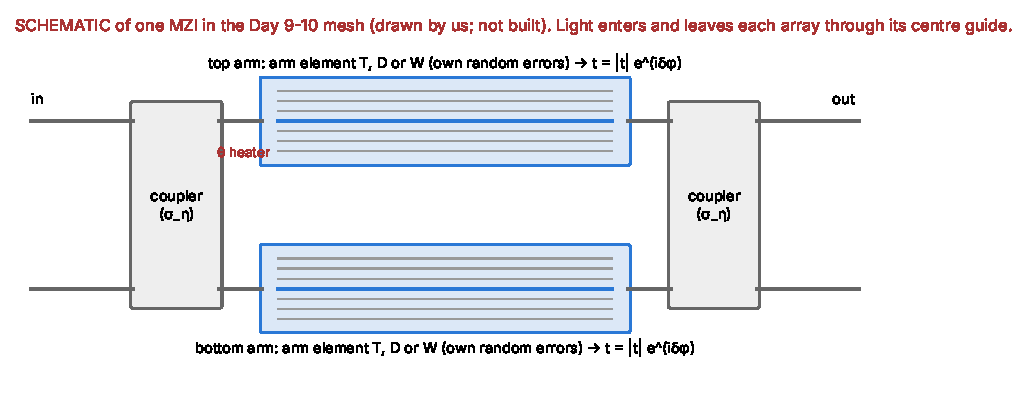
\includegraphics[width=0.9\linewidth]{../../figures/fig_bridge_schematic.pdf}
\caption{\textbf{Schematic drawn by us} of one MZI of the simulated mesh (not built).}
\label{fig:sch}
\end{figure}

%=====================================================================
\section{Theory: from arm errors to circuit fidelity \evd{Derived; Verified-by-test}}
%=====================================================================
Each arm error acts on one mode inside the mesh. From Day 8, a phase error of size $s$ on one mode costs $(N-1)s^2/N^2$ of fidelity. A \emph{log-amplitude} error $a=\ln|t|$ of the same size costs the same: with $W=e^{aP}$, $\mathrm{Tr}W\approx N+a+\frac{a^2}{2}$ and $\mathrm{Tr}W^\dagger W\approx N+2a+2a^2$, so $F\approx1-(N-1)a^2/N^2$. A mesh has $N(N-1)$ internal arms, so
\[
\boxed{1-F\approx\frac{(N-1)^2}{N}\Big[\sigma_{\delta\varphi}^2+\sigma_{\ln|t|}^2\Big]+2(N-1)\,\sigma_\eta^2 .}
\]
The test \texttt{test\_arm\_amplitude\_error\_counts\_like\_phase\_error} checks the equal cost (within 10\%). In the Monte Carlo, this formula (fed with the measured arm statistics) agrees with the full mesh simulation to a few per cent whenever $1-F<0.1$; above that, $F$ saturates and the first-order formula over-estimates.

\textbf{Arm coefficients} measured from 4000 arms at $\sigma=0.003$ (per unit $\sigma$; $L=10$ coupling lengths $=15.7/\kc$):
\begin{tabular}{@{}lcccc@{}}\toprule
 & \multicolumn{2}{c}{gap error $\sigma_\kappa$} & \multicolumn{2}{c}{on-site error $\sigma_\beta$}\\
 & phase & log-amplitude & phase & log-amplitude\\\midrule
T & $7\times10^{-13}$ (zero) & 0.77 & 12.4 & 0.02\\
D & 8.1 & 0.19 & 13.1 & 0.32\\
W & 0 & 0 & 15.6 ($=L$) & 0\\\bottomrule
\end{tabular}
\smallskip

D's gap-phase coefficient $8.1\approx0.51\times15.7$ and W's on-site coefficient $=L$ match Days 3--6. T converts gap errors \emph{entirely} into amplitude (0.77 per unit $\sigma_\kappa$), as Day 6 found.

%=====================================================================
\section{Results}
%=====================================================================
\begin{figure}[t]\centering
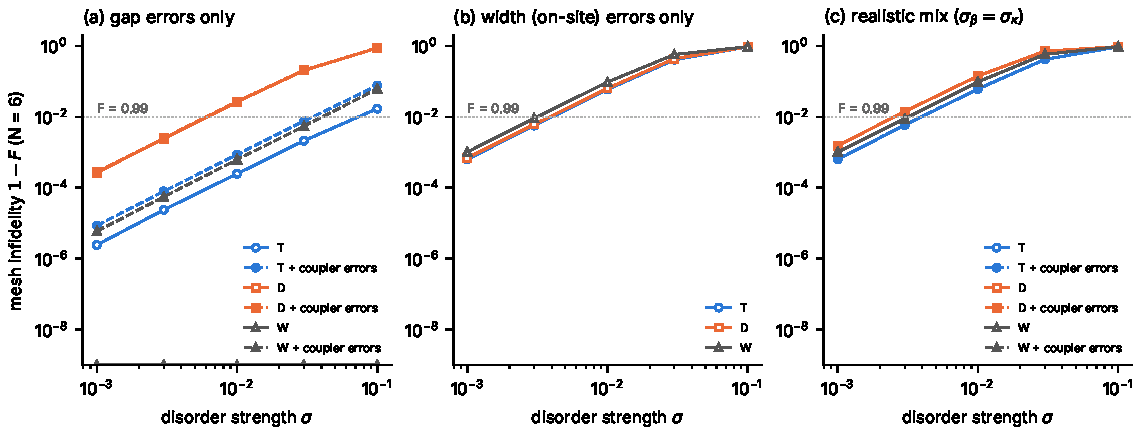
\includegraphics[width=\linewidth]{../../figures/fig_bridge.pdf}
\caption{\textbf{Simulation}, \texttt{scripts/day9\_bridge.py} $\to$ \texttt{data/day9\_bridge.npz}. Mesh infidelity vs.\ disorder strength. Open markers: arm errors only; filled: arms + coupler gap errors. W with gap errors in the arms only is exactly zero (drawn at the bottom edge).}
\label{fig:bridge}
\end{figure}

\begin{tabular}{@{}lccc@{}}\toprule
Mesh infidelity $1-F$ ($N=6$), $\sigma=0.01$ & T & D & W\\\midrule
gap errors, arms only & $2.5\times10^{-4}$ & $0.027$ & $0$\\
gap errors, arms + couplers & $8.7\times10^{-4}$ & $0.027$ & $6.2\times10^{-4}$\\
on-site (width) errors & $0.060$ & $0.064$ & $0.097$\\
realistic mix ($\sigma_\beta=\sigma_\kappa$), arms + couplers & $0.062$ & $0.144$ & $0.098$\\\bottomrule
\end{tabular}
\smallskip

\begin{enumerate}[itemsep=2pt]
\item \textbf{Against gap errors, the array-level protection does reach the circuit.} T is about 100$\times$ better than D. Its small remaining infidelity comes from \emph{amplitude} errors, not phase.
\item \textbf{But a plain waveguide is as good or better.} W has no couplings, so gap errors in the arms cannot touch it at all. Once the couplers' own gap errors are included, T and W are equal within 40\% --- the couplers set the floor for both.
\item \textbf{Against width errors, nothing is protected.} T and D are equal; both are about 0.6$\times$ W. That gain is \emph{not} topological: a mode spread over several guides averages their random errors ($\sqrt{\mathrm{IPR}}=0.81$), and D gets the same gain.
\item \textbf{In the realistic mix, T is best} (0.062 vs.\ D 0.144 and W 0.098), but the margin over W comes from mode spreading, and its size depends on the unknown ratio $\sigma_\beta/\sigma_\kappa$.
\end{enumerate}

\subsection{The design map: where is $F\ge0.99$?}
\begin{figure}[h]\centering
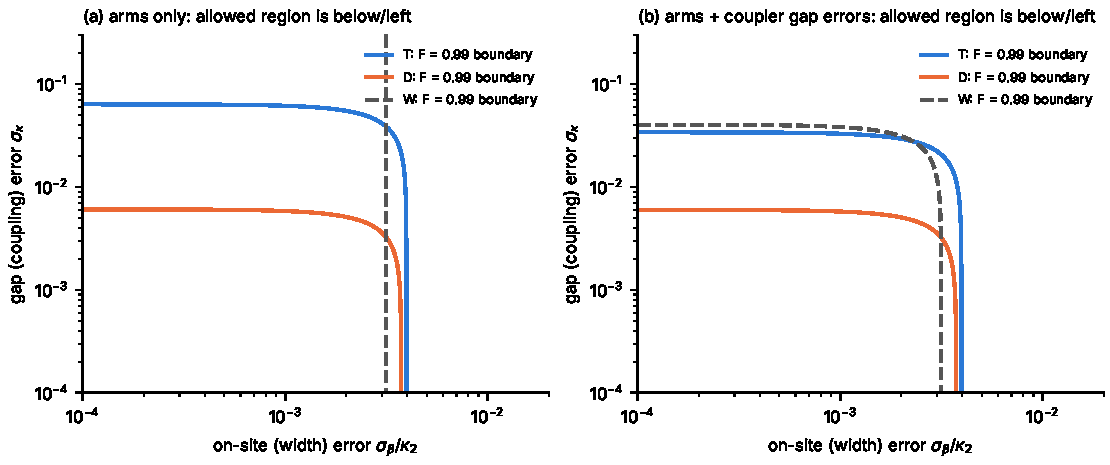
\includegraphics[width=\linewidth]{../../figures/fig_design_map.pdf}
\caption{First-order model with the measured arm coefficients: boundary $F=0.99$ for independent on-site and gap errors. Allowed region: below and to the left of each line.}
\label{fig:map}
\end{figure}
Read from Fig.~\ref{fig:map} \evd{Derived from the calibrated model}:
\begin{itemize}[itemsep=1pt]
\item \textbf{Width errors decide everything}: every element needs $\sigma_\beta\lesssim0.004\,\kc$ at this length (W: $0.0032\kc$). Halving the arm length doubles this tolerance ($\delta\varphi\propto L$).
\item \textbf{Gap tolerance}, arms only: T $\approx0.065$, D $\approx0.006$, W unlimited. With coupler errors: T $\approx0.035$, W $\approx0.04$, D $\approx0.006$.
\end{itemize}

\subsection{A cost that fidelity hides: insertion loss}
A clean T arm delivers only $|a_c(L)|^2=0.694$ of its input to the output guide (D: 0.633; W: 1). The rest stays spread in the array's other guides --- on a real chip it is lost light. A path through an $N=6$ mesh passes 6 arms: $0.694^6\approx0.11$ of the light survives (D: $0.064$). Normalised fidelity ignores uniform loss by construction, so this must be reported separately. \evd{Simulated (clean values) + arithmetic}

%=====================================================================
\section{Answer to the research question (for this model)}
%=====================================================================
\note{\textbf{Does topological protection of optical transport also protect interferometric phase?}\\
\textbf{Partly, and only for one error channel.} For errors that preserve chiral symmetry (gap/coupling errors), the topological mode's phase is protected exactly --- in the eigenvalue (Day 4), in the arm-to-arm phase (Day 6), and in the fidelity of a whole MZI mesh (Days 9--10). The protection does not remove those errors: it moves them into the amplitude, which still costs fidelity. For errors that break chiral symmetry (width/propagation-constant errors, which dominate the tolerance), there is no protection at all. And for the protected channel, a plain uncoupled waveguide achieves the same immunity without the topological array's insertion loss.}

\textbf{Physically bounded design criterion (for the paper).} A topological array is worth using as an interferometer arm only if (i) coupled guides are unavoidable (e.g.\ dense packing where neighbours couple anyway), (ii) gap errors dominate width errors ($\sigma_\kappa$ large compared with $\sigma_\beta L$), and (iii) its insertion loss is acceptable or solved by a better input/output design. Otherwise, a plain waveguide is the better arm. In all cases the tolerance is set by
\[
1-F\approx\frac{(N-1)^2}{N}\big[(c_\beta\sigma_\beta L)^2+(c_\kappa\sigma_\kappa)^2\big]+2(N-1)\big(\tfrac\pi4\sigma_\kappa\big)^2,
\]
with $c_\beta=\sqrt{\mathrm{IPR}}\approx0.8$ (arrays) or 1 (plain guide), and $c_\kappa=0.77$ (T, amplitude only), $\approx8.1$ (D, mostly phase; $=0.51\,\kc L$ at this length), 0 (W). These numbers are for $N=6$, $L=10$ coupling lengths and $\kappa_1/\kappa_2=1/3$.

%=====================================================================
\section{Limitations of this bridge (must appear in the paper)}
%=====================================================================
\begin{enumerate}[itemsep=1pt]
\item Assumption A-bridge: centre-guide in/out, one element per arm. Other ways of using a topological array in a circuit (e.g.\ the array \emph{as} the coupler) were not studied.
\item Nearest-neighbour coupled-mode model; L1 (end/edge self-shift), L2 (next-nearest coupling) neglected.
\item Errors independent from arm to arm; no wafer-scale gradients or correlated errors between neighbouring arms (these would partly cancel inside each MZI).
\item Absolute $\kappa$ and the ratio $\sigma_\beta/\sigma_\kappa$ are unknown, so tolerances are in units of $\kc$, not nanometres.
\item Random mesh settings, not a decomposition of a chosen target; $N=6$ only (the $N$-scaling is given by the formula).
\item No thermal crosstalk, heater drift, wavelength dependence or detector noise.
\end{enumerate}

%=====================================================================
\section{Hardware}
%=====================================================================
The images in our chat (published work, not ours) show integrated MZI chips and quantum photonic circuits built from the same components: directional couplers, heater phase shifters and waveguide arms. We found no published device that places SSH arrays inside the arms of an MZI mesh; the architecture here is a numerical proposal. Before stating ``no such device exists'' in the paper, do a proper literature search (record it in the literature matrix).

\section{Code and tests}
New: \texttt{topq/bridge.py} (arm pools, insertion loss, mesh with arm errors, first-order prediction, \texttt{run\_bridge}); \texttt{scripts/day9\_bridge.py} (290~s), \texttt{scripts/day9\_arm\_schematic.py}; \texttt{tests/test\_bridge.py} (9 tests). Suite: \textbf{128 passed}.

\section{Self-test}
\begin{enumerate}[itemsep=1pt]
\item Why is the plain waveguide W the right control, and what does it show?
\item Show that a small log-amplitude error costs the same fidelity as a phase error of the same size.
\item Why is T 100$\times$ better than D under gap errors, but equal to D under width errors?
\item Why does T's advantage over W under width errors not count as topological?
\item Why does normalised fidelity hide the insertion loss, and how big is it here?
\item State the design criterion in two sentences.
\end{enumerate}
\end{document}
